\relatorio{Taxa de juros neutra para o Brasil e Estados Unidos}
    {\noindent Pesquisadores: Giovanni Vescovi Filho, Camila Vaz}
    {Devido às recentes notícias e observações de elevados juros reais ex-Ante, buscamos entender o comportamento do juros e se o mesmo encontra-se em um valor alto demais ou não seguindo abordagens mais simples de mensuração, como a regra de taylor e um modelo VAR. Após os modelos e seus resultados, algumas das justificativas para os valores são variáveis de difícil mensuração e de modelagem mais difícil ainda.}
    {Juros, Política Monetária, Brasil, Estados Unidos, VAR e Regra de Taylor
    }

\section*{Introdu\c{c}\~{a}o e motiva\c{c}\~{a}o }

 No presente trabalho, foi desenvolvido um m\'{e}todo para determinar a taxa de juros neutra de um pa\'{i}s atrav\'{e}s da Regra de Taylor (\textit{Taylor Rule}). A determina\c{c}\~{a}o da taxa de juros neutra ainda \'{e} um tema te\'{o}rico com aplica\c{c}\~{o}es diferentes no mundo atual por seus diferentes m\'{e}todos de determina\c{c}\~{a}o. Tal taxa consiste naquela capaz de fazer com que o PIB de um pa\'{i}s convirja ao seu potencial simultaneamente ancorando a pol\'{i}tica monet\'{a}ria. Visto isso, sua aplica\c{c}\~{a}o apresentada nesse trabalho, consistir\'{a} na compara\c{c}\~{a}o da taxa de juros real efetiva de um pa\'{i}s com a taxa neutra a fim de determinar distor\c{c}\~{o}es presentes nas economias apresentadas.

A maior motiva\c{c}\~{a}o para o desenvolvimento de dada pesquisa foi a disparidade entre a taxa de juros efetiva brasileira comparada internacionalmente.

\begin{figure}
    \centering
    \caption{Taxa de Juros Real (Média Taxa Ex-Post 2012-2016 - \%a.a.)}
    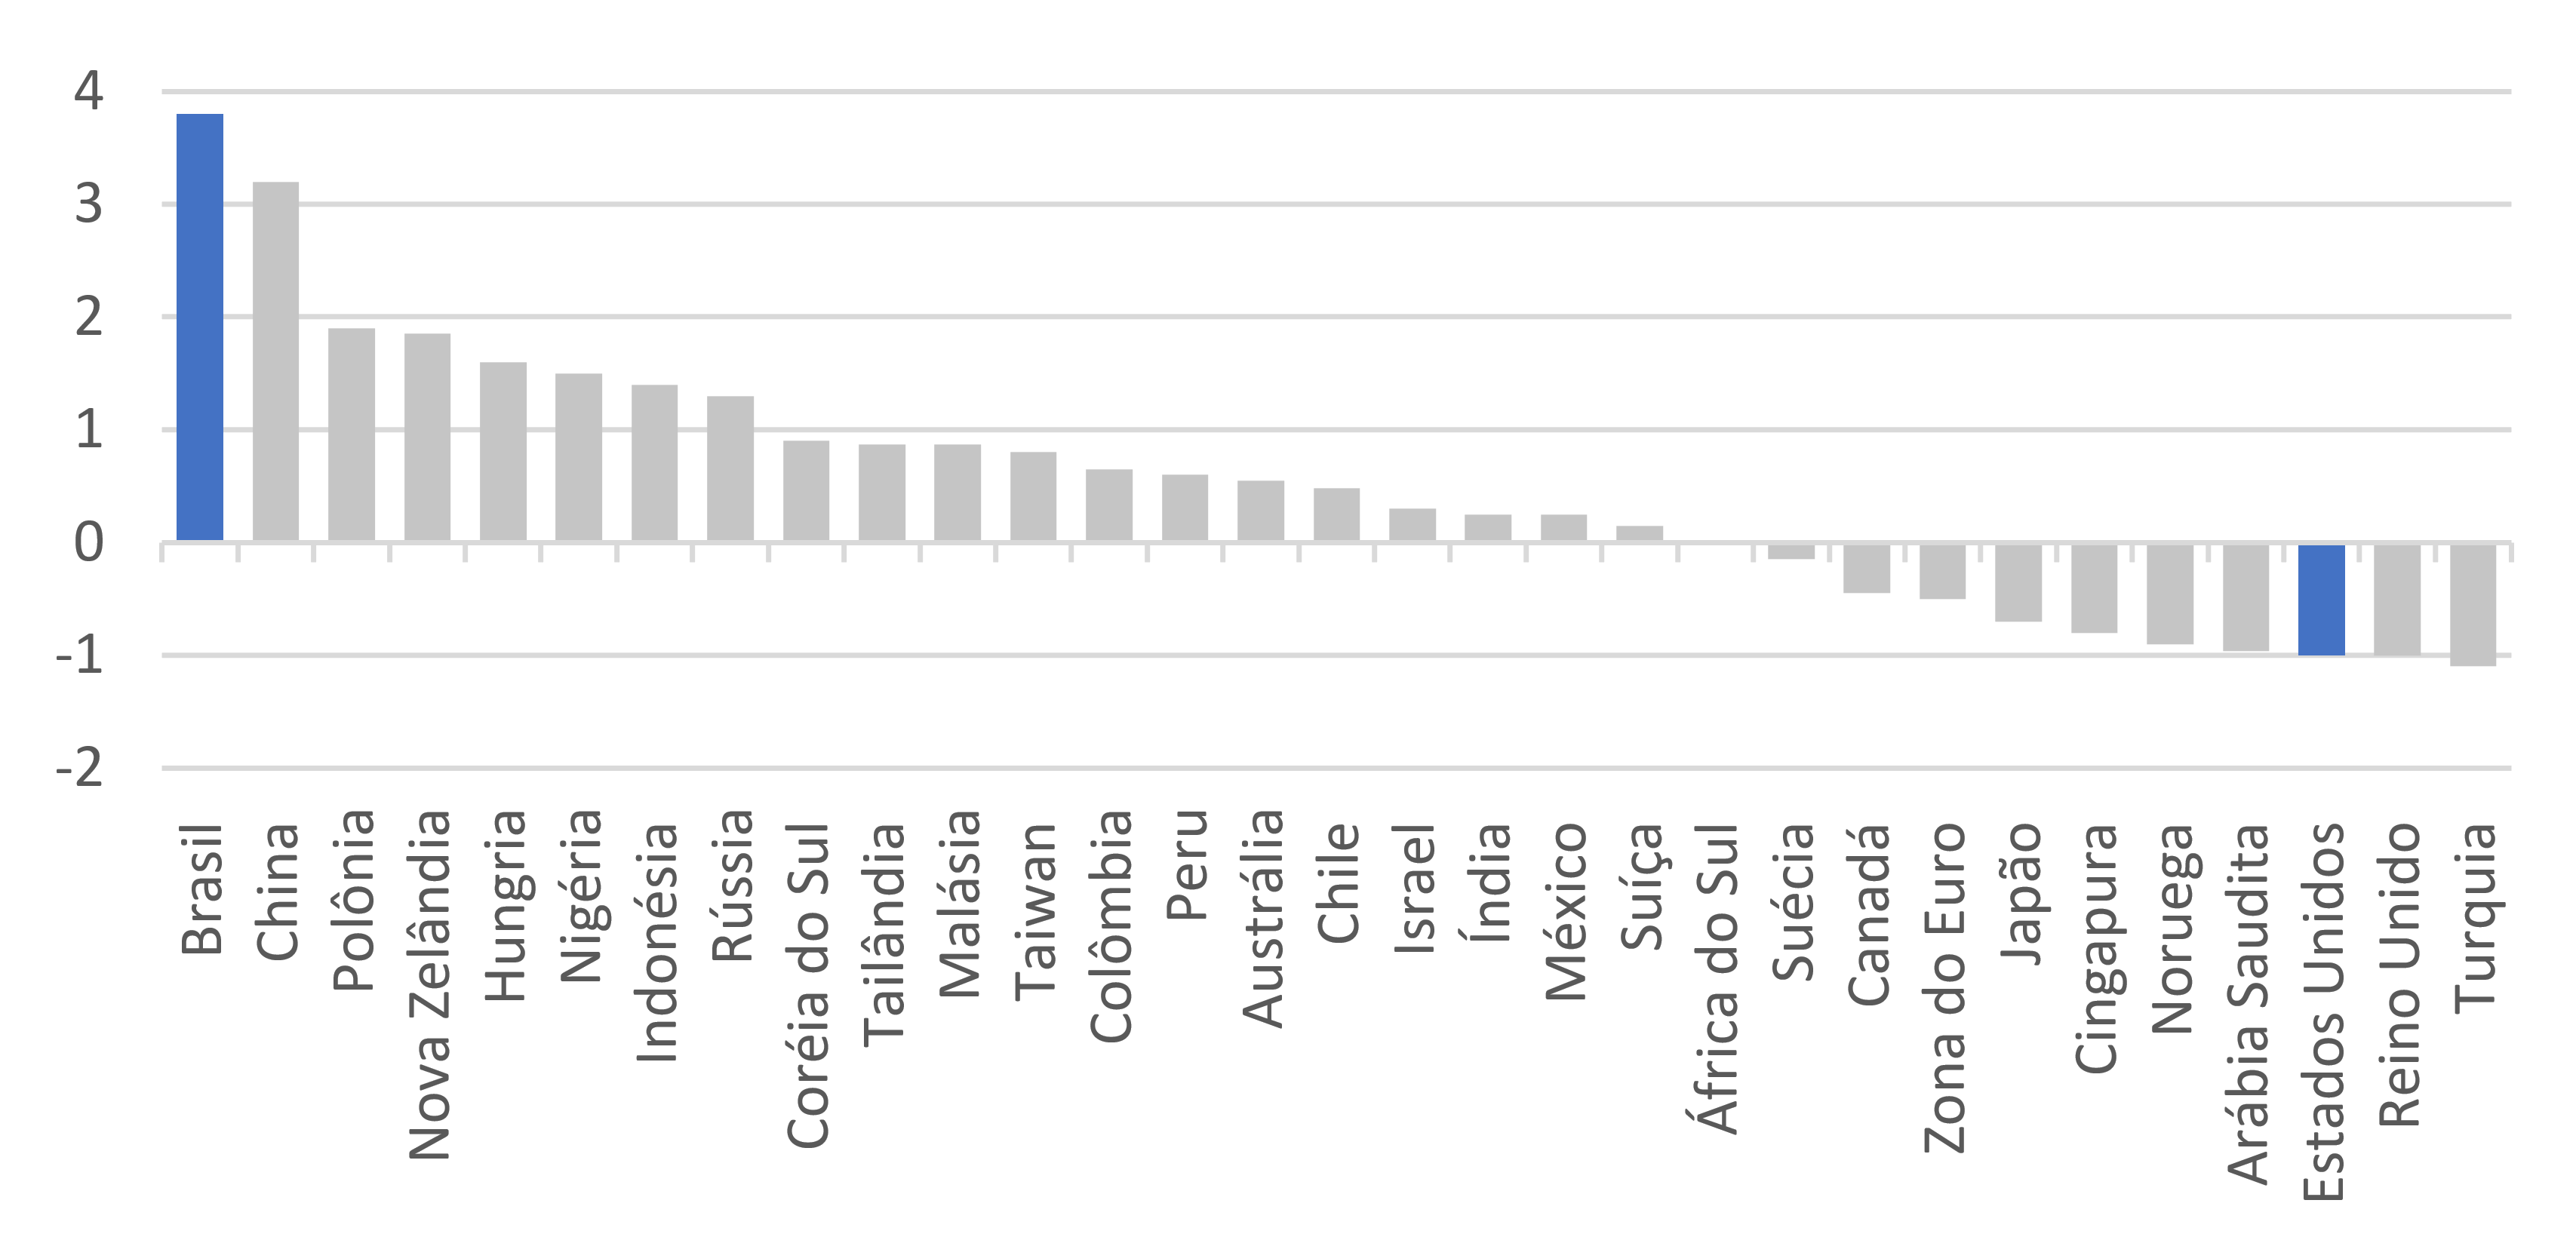
\includegraphics[width = \linewidth]{relatorios/macro/imagens/grafico1}
    \subcaption{Fonte: \cite{itau}}
\end{figure}

 Como pode ser observado no Gr\'{a}fico 1, nesta compara\c{c}\~{a}o, o Brasil \'{e} o pa\'{i}s com a maior taxa de juros real no per\'{i}odo de 2012 a 2016. Dessa forma, o objetivo deste trabalho ser\'{a}, atrav\'{e}s de uma an\'{a}lise hist\'{o}rica de dados, observar distor\c{c}\~{o}es nas taxas de juros brasileiras e determinar hip\'{o}teses para tais ao compararmos com um pa\'{i}s com uma economia est\'{a}vel, como os Estados Unidos. Analogamente, ser\'{a} utilizado este pa\'{i}s como um ``grupo de controle'' a fim de estipularmos distor\c{c}\~{o}es. 

\section*{Dados e \textit{Taylor Rule} }

 Primeiramente, necessita-se determinar uma f\'{o}rmula padr\~{a}o a fim de encontrarmos duas taxas de juros neutras, tanto para o Brasil como para os Estados Unidos. Para isso, foi utilizada a Regra de Taylor que consiste em um c\'{a}lculo para pol\'{i}tica macroecon\^{o}mica capaz de determinar a taxa de juros ideal para um pa\'{i}s em fun\c{c}\~{a}o da infla\c{c}\~{a}o e do volume da atividade econ\^{o}mica, com isso, um de seus \textit{inputs} \'{e} a taxa de juros real de equil\'{i}brio, somada \`{a} um pr\^{e}mio de risco que reflete as expectativas futuras de infla\c{c}\~{a}o e outros riscos. Para este trabalho em quest\~{a}o, tal taxa real de equil\'{i}brio, definida por Taylor como tal por representar o n\'{i}vel da taxa de juros necess\'{a}rio para manter a economia em seu pleno emprego e estabilidade de pre\c{c}os, ser\'{a} a nossa taxa neutra. 

 Analogamente com uma simples manipula\c{c}\~{a}o da f\'{o}rmula obtemos: 

Taylor Rule: 
\[i=r+~\pi +0,5*\left(\pi -{\pi }^T\right)+0,5*\left(y-y^{PE}\right)\] 

Isolar r: 
\[r=~i-\pi -0,5*\left(\pi -{\pi }^T\right)-0,5*\left(y-y^{PE}\right)\] 


\begin{itemize}
\item  $i=Juros~real$

\item  $r=Juros~nominal$\textit{ de equil\'{i}brio }

\item  $\pi =Infla\textrm{\c{c}}\textrm{\~{a}}o$

\item  ${\pi }^T=meta~de~infla\textrm{\c{c}}\textrm{\~{a}}o~$

\item  $y=PIB$

\item  $y^{PE}=PIB~potencial$
\end{itemize}

A taxa de juros real definida acima por $i$, consiste na taxa efetiva de juros de determinado pa\'{i}s descontada a infla\c{c}\~{a}o, j\'{a} a taxa de juros nominal consiste na taxa de juros sem o desconto da infla\c{c}\~{a}o. 

\section*{Modelagem}

Para realiza\c{c}\~{a}o do c\'{a}lculo temporal da taxa neutra pela f\'{o}rmula, foi importando cada vari\'{a}vel dos sites dos bancos centrais respectivos de cada pa\'{i}s, bastou apenas col\'{a}-los respectivamente na f\'{o}rmula estipulada e, atrav\'{e}s de uma planilha do Excel, construiu-se uma nova vari\'{a}vel temporal que pode ser incorporada nos gr\'{a}ficos a seguir. \'{E} importante ressaltar que para a meta infla\c{c}\~{a}o dos EUA foi utilizada a s\'{e}rie \textit{10-Year Breakeven Inflation Rate }que consiste na expectativa de infla\c{c}\~{a}o futura baseada no rendimento at\'{e} o vencimento de t\'{i}tulos do Tesouro de 10 anos. \textbf{}

 Como inputs para as f\'{o}rmulas supracitadas temos que para o Brasil, os dados utilizados como taxa de juros, infla\c{c}\~{a}o e hiato do produto (diferen\c{c}a entre produto observado e potencial) foram a Selic [432], IPCA [433] e IBC-br[24364]. 

 J\'{a} para os Estados Unidos, o que foi adquirido foram as s\'{e}ries temporais de: ``Gross Domestic Product, Billions of Dollars, Quarterly, Seasonally Adjusted Annual Rate'' (GDP), ``Real Potential Gross Domestic Product, Billions of Chained 2012 Dollars, Quarterly, Not Seasonally Adjusted'' (GDPPOT), ``Federal Funds Effective Rate, Percent, Quarterly, Not Seasonally Adjusted'' (DFF), ``Sticky Price Consumer Price Index less Food and Energy, Percent Change from Year Ago, Quarterly, Seasonally Adjusted'' (CORESTICKM159SFRBATL), ``10-Year Breakeven Inflation Rate, Percent, Quarterly, Not Seasonally Adjusted'' (T10YIE). 

\section*{\textit{R Studio}}

 Diferentemente do que foi feito no Excel, no RStudio, o m\'{e}todo de estima\c{c}\~{a}o da vari\'{a}vel de interesse ser\'{a} de Vetor Autorregressivo (VAR).

 Para isso, as s\'{e}ries temporais de interesse, similarmente ao Excel, ser\~{a}o taxa de juros, infla\c{c}\~{a}o e hiato do produto tamb\'{e}m tendo como c\'{o}digos, da base de dados de s\'{e}ries temporais do Banco Central brasileiro, os valores 432, 433 e 24364. 

 Ap\'{o}s a coleta do Brasil, foi feita a dos Estados Unidos, desta vez tendo como fonte dos dados o banco de dados do FRED de St. Louis. Referente \`{a} infla\c{c}\~{a}o, taxa de juros e PIB, os c\'{o}digos da base foram CPIAUCSL, DFF e GDP.

 Em termos de instrumentaliza\c{c}\~{a}o pr\'{a}tica, para ambos os pa\'{i}ses foram feitos os mesmos procedimentos, sejam de passo a passo seja de determina\c{c}\~{a}o de frequ\^{e}ncia desejada, trimestral. 


 Com isso, primeiro para se extrair o hiato do produto, foi utilizado o filtro Hodrick-Prescott (HP), para poder extrair a tend\^{e}ncia da s\'{e}rie, simbolizando o produto potencial, e os desvios da tend\^{e}ncia, os ciclos, que representam os hiatos do produto. 

\section*{Primeiros passos estima\c{c}\~{a}o}

\textit{ }Ap\'{o}s a consolida\c{c}\~{a}o das vari\'{a}veis de interesse, e realizando os devidos testes, entendeu-se que tomar a diferen\c{c}a do logaritmo da s\'{e}rie, para os \'{i}ndices de pre\c{c}o, transformando-os em infla\c{c}\~{a}o, seria o mais apropriado. 

 Ap\'{o}s a estima\c{c}\~{a}o do VAR, entende-se que, ap\'{o}s a verifica\c{c}\~{a}o da matriz de correla\c{c}\~{a}o dos res\'{i}duos, como os res\'{i}duos de cada equa\c{c}\~{a}o s\~{a}o correlacionados no mesmo espa\c{c}o de tempo, que os valores das matrizes de coeficientes n\~{a}o s\~{a}o interpret\'{a}veis. Por\'{e}m, como o intuito do trabalho n\~{a}o \'{e} verificar a intensidade das rela\c{c}\~{o}es das vari\'{a}veis entre si e sim apenas o n\'{i}vel dos juros isso n\~{a}o \'{e} um problema. 

\section*{Conclus\~{o}es e resultados }

\subsection*{\textit{R Studio}}

A respeito dos resultados do m\'{e}todo VAR, tem-se que o n\'{i}vel de juros dos \'{u}ltimos per\'{i}odos est\'{a} dentro do intervalo de confian\c{c}a observado, por\'{e}m, como os intervalos de confian\c{c}a possuem bandas muito largas, estes resultados s\~{a}o pouco conclusivos, tanto de maneira positiva quanto negativamente.

Tendo como visualiza\c{c}\~{a}o gr\'{a}fica dos resultados Brasil do R Studio:

\begin{figure}
    \centering
    \caption{Backtesting BRA}
    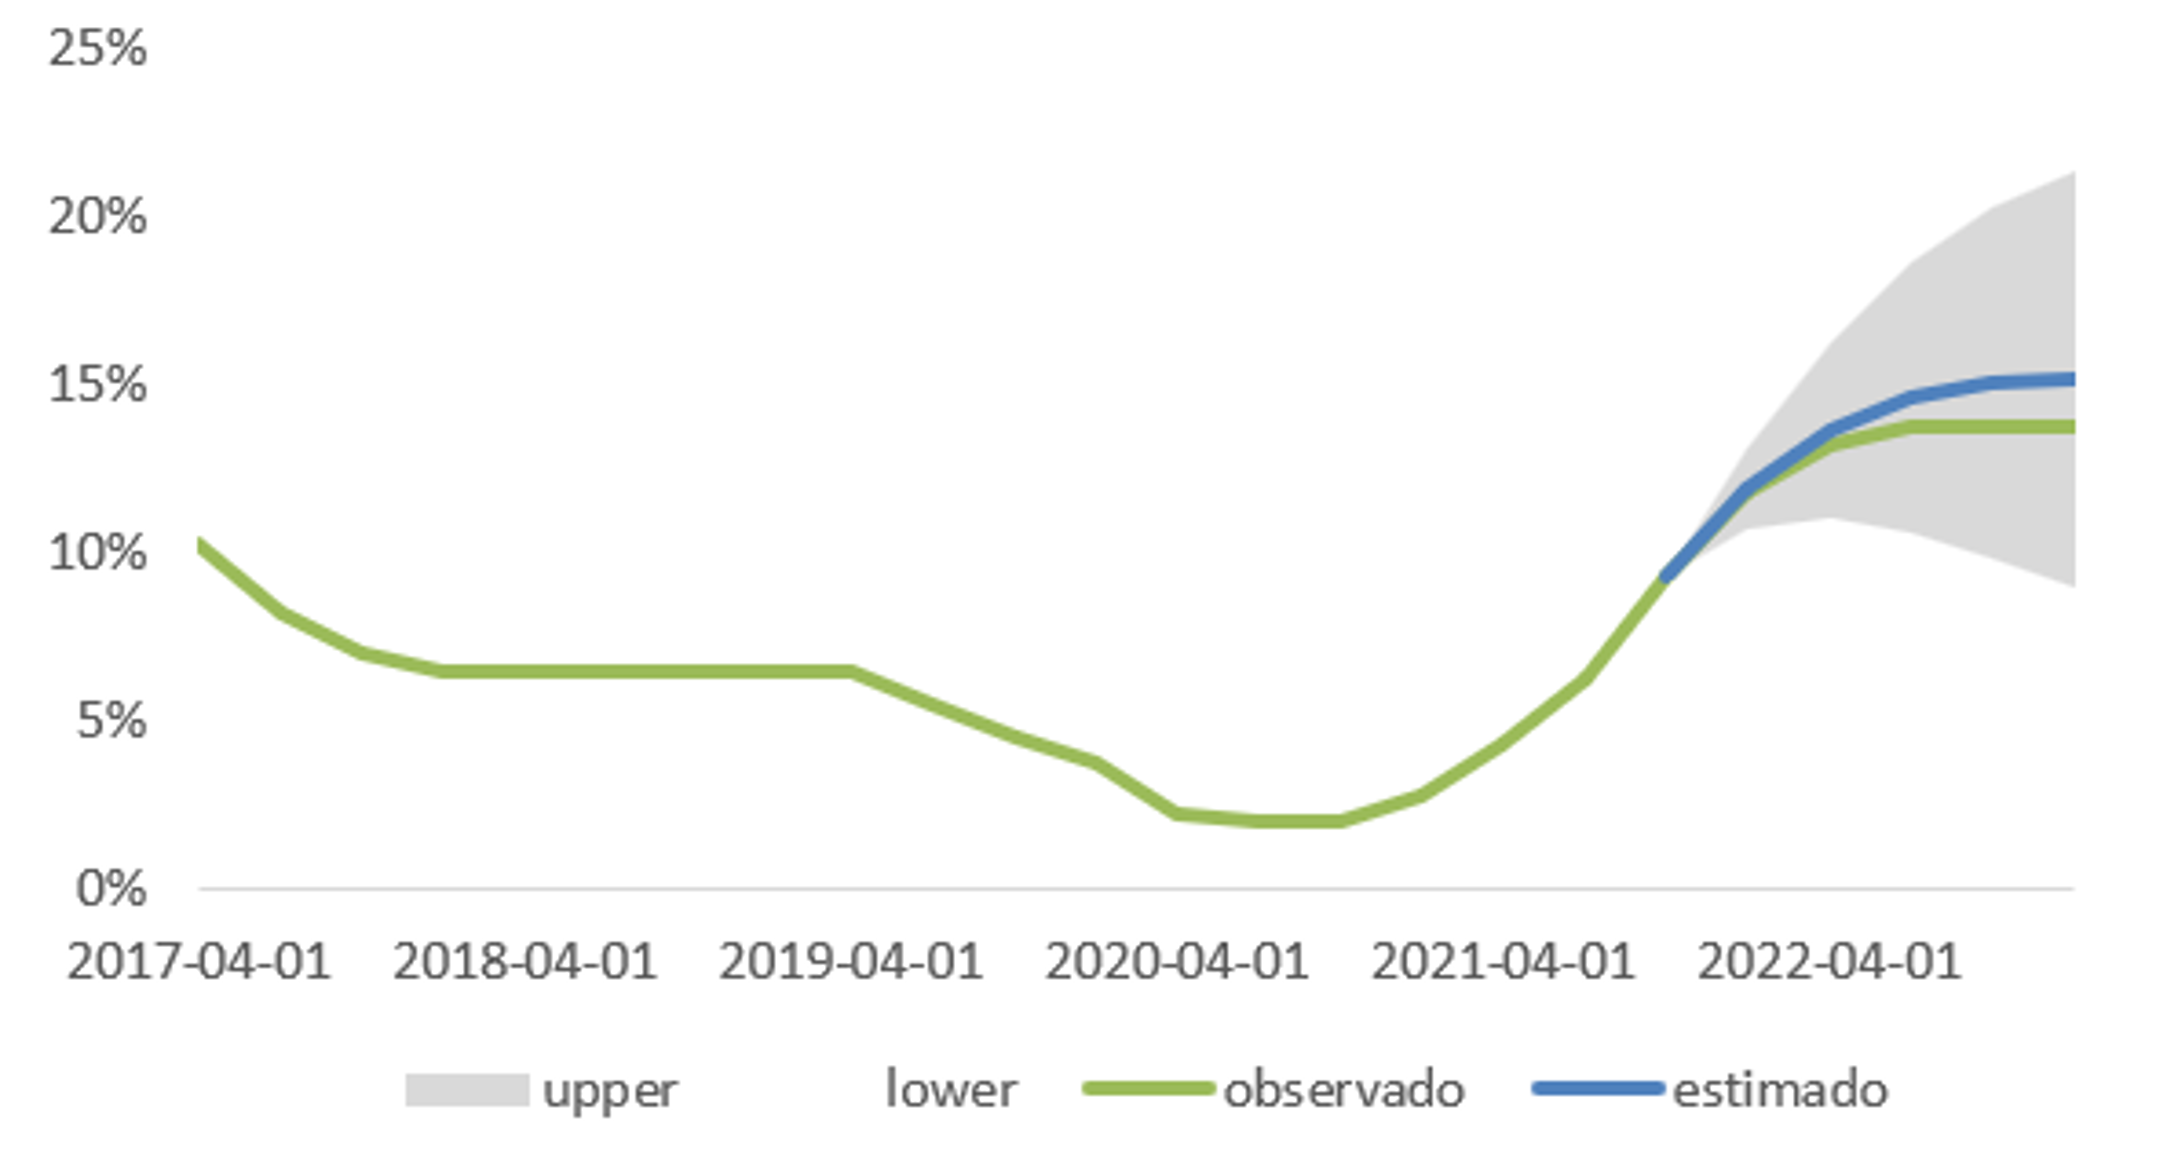
\includegraphics[width = 0.75\linewidth]{relatorios/macro/imagens/grafico2}
\end{figure}


J\'{a} os resultados dos USA do R Studio:


\begin{figure}
    \centering
    \caption{Backtesting USA}
    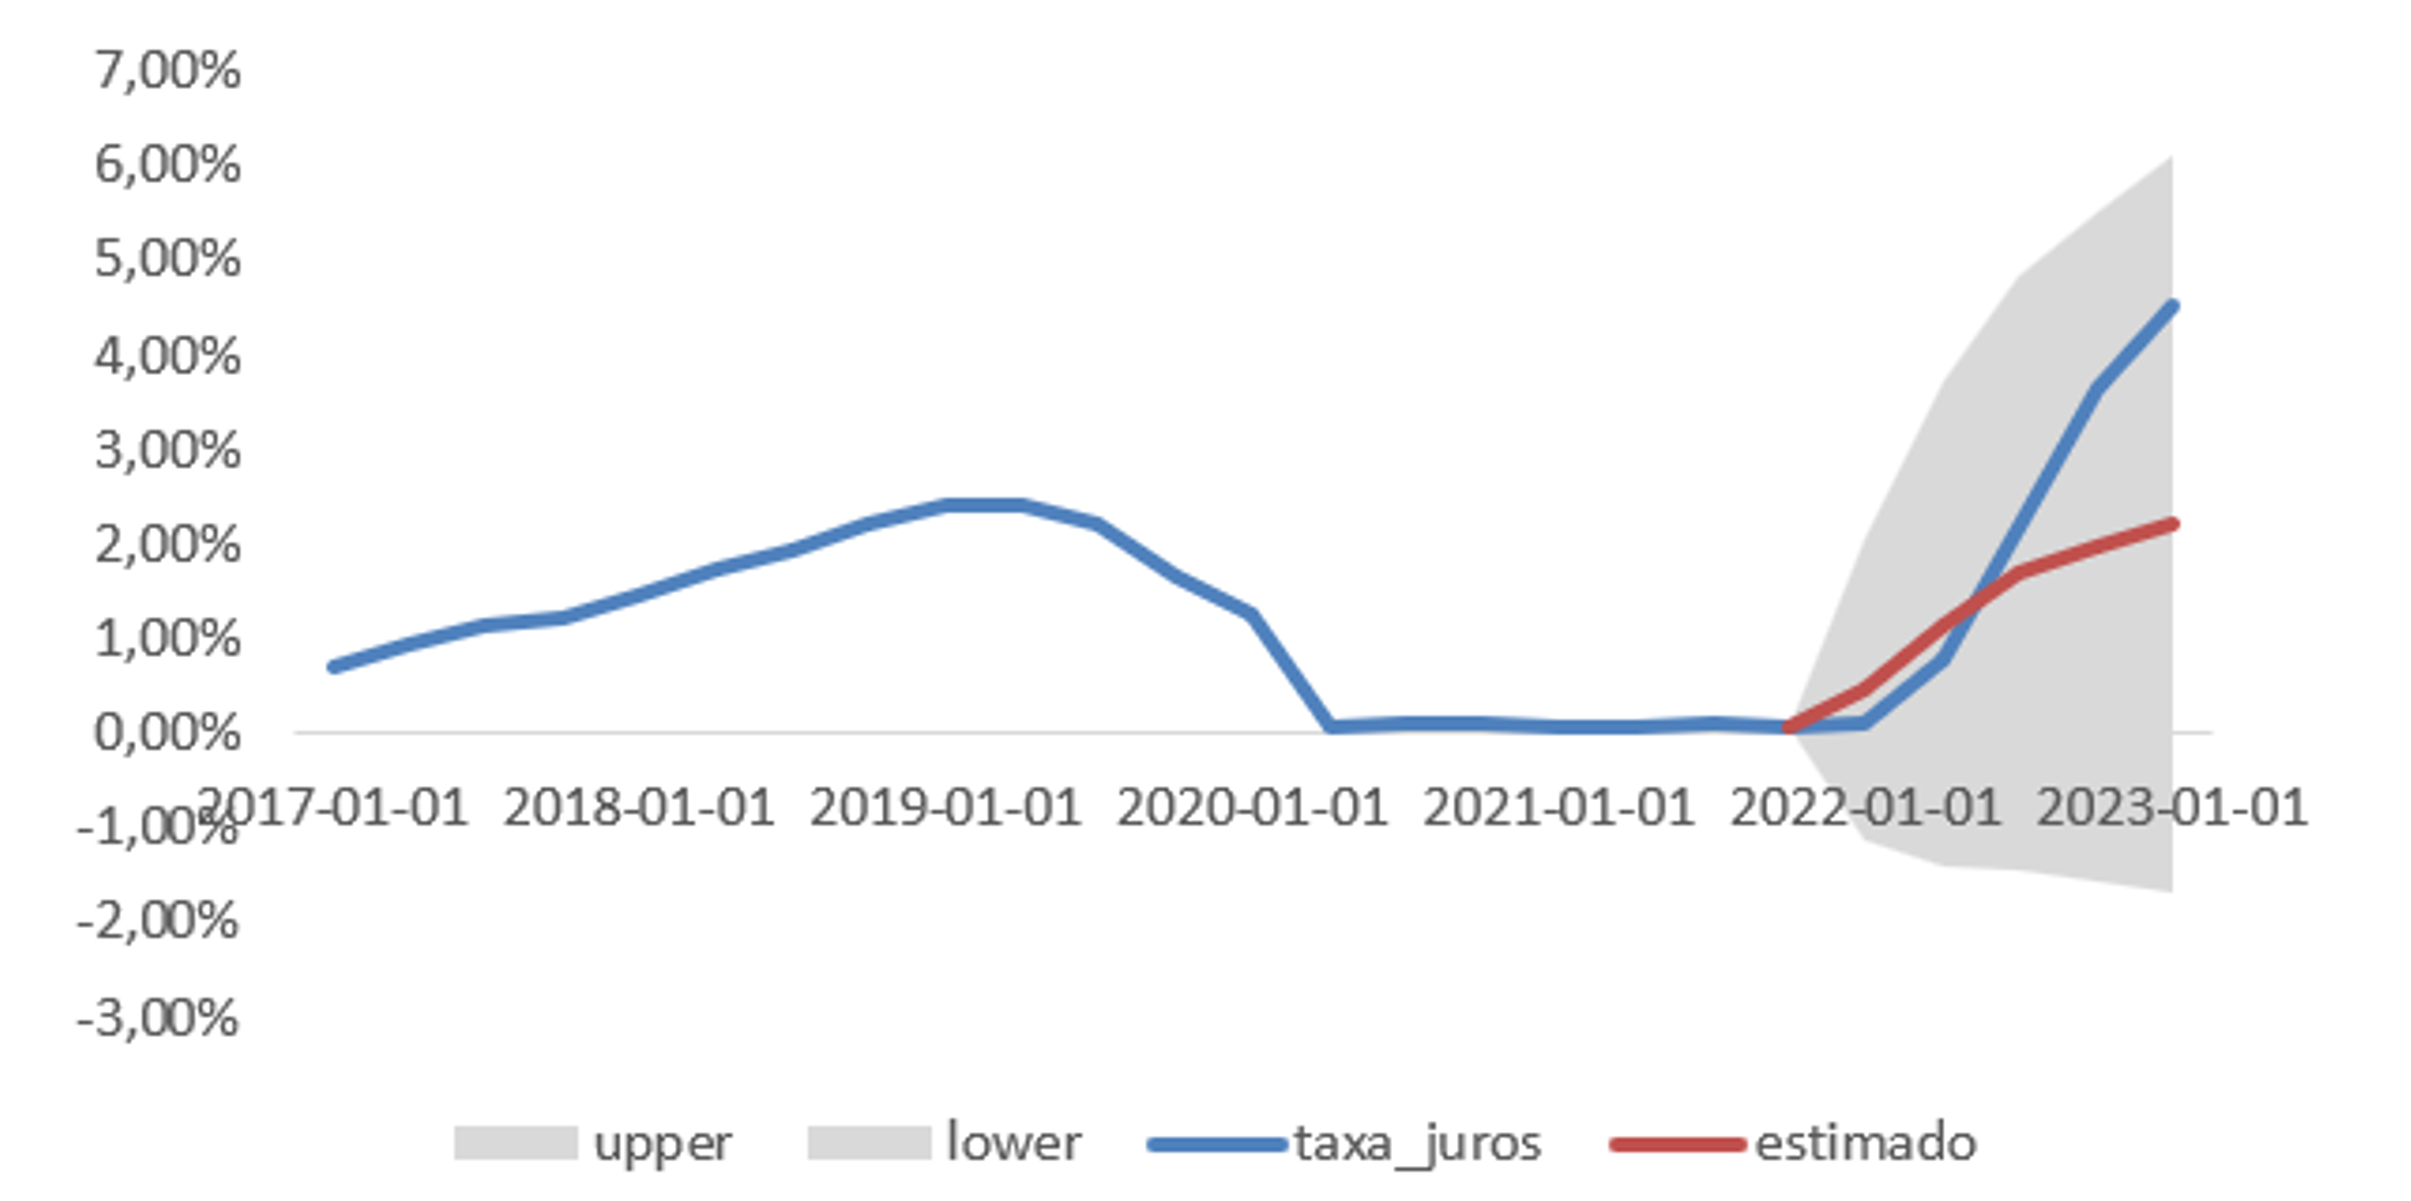
\includegraphics[width = 0.75\linewidth]{relatorios/macro/imagens/grafico3}
\end{figure}


 Como \'{e} poss\'{i}vel ver, graficamente, os intervalos de confian\c{c}a s\~{a}o muito grandes, tanto para os USA quanto para o Brasil, neste sentido, algumas das explica\c{c}\~{o}es \'{e} o impacto da recente crise da pandemia, algo que modelos n\~{a}o s\~{a}o capazes de representar a real discricionariedade necess\'{a}ria para resolver as quest\~{o}es correntes. Sendo assim, os par\^{a}metros e as estimativas aproximam-se mais de ru\'{i}dos do que de sinal para a nossa an\'{a}lise. Sendo assim, deixamos em segundo plano as an\'{a}lises e resultados gerados a partir do uso do RStudio e do Vetor Autorregressivo. \textbf{}

\subsection*{\textit{Excel}}

Dada as interpreta\c{c}\~{o}es e resultados gerados pelo RStudio, optou-se por dar mais destaque e maior peso para os resultados do Excel para o c\'{a}lculo da taxa de juros e suas consequentes interpreta\c{c}\~{o}es. 

 Portanto, obtivemos os seguintes resultados gr\'{a}ficos: 

 \begin{figure}
    \centering
    \caption{Taxas de juros brasileiras}
    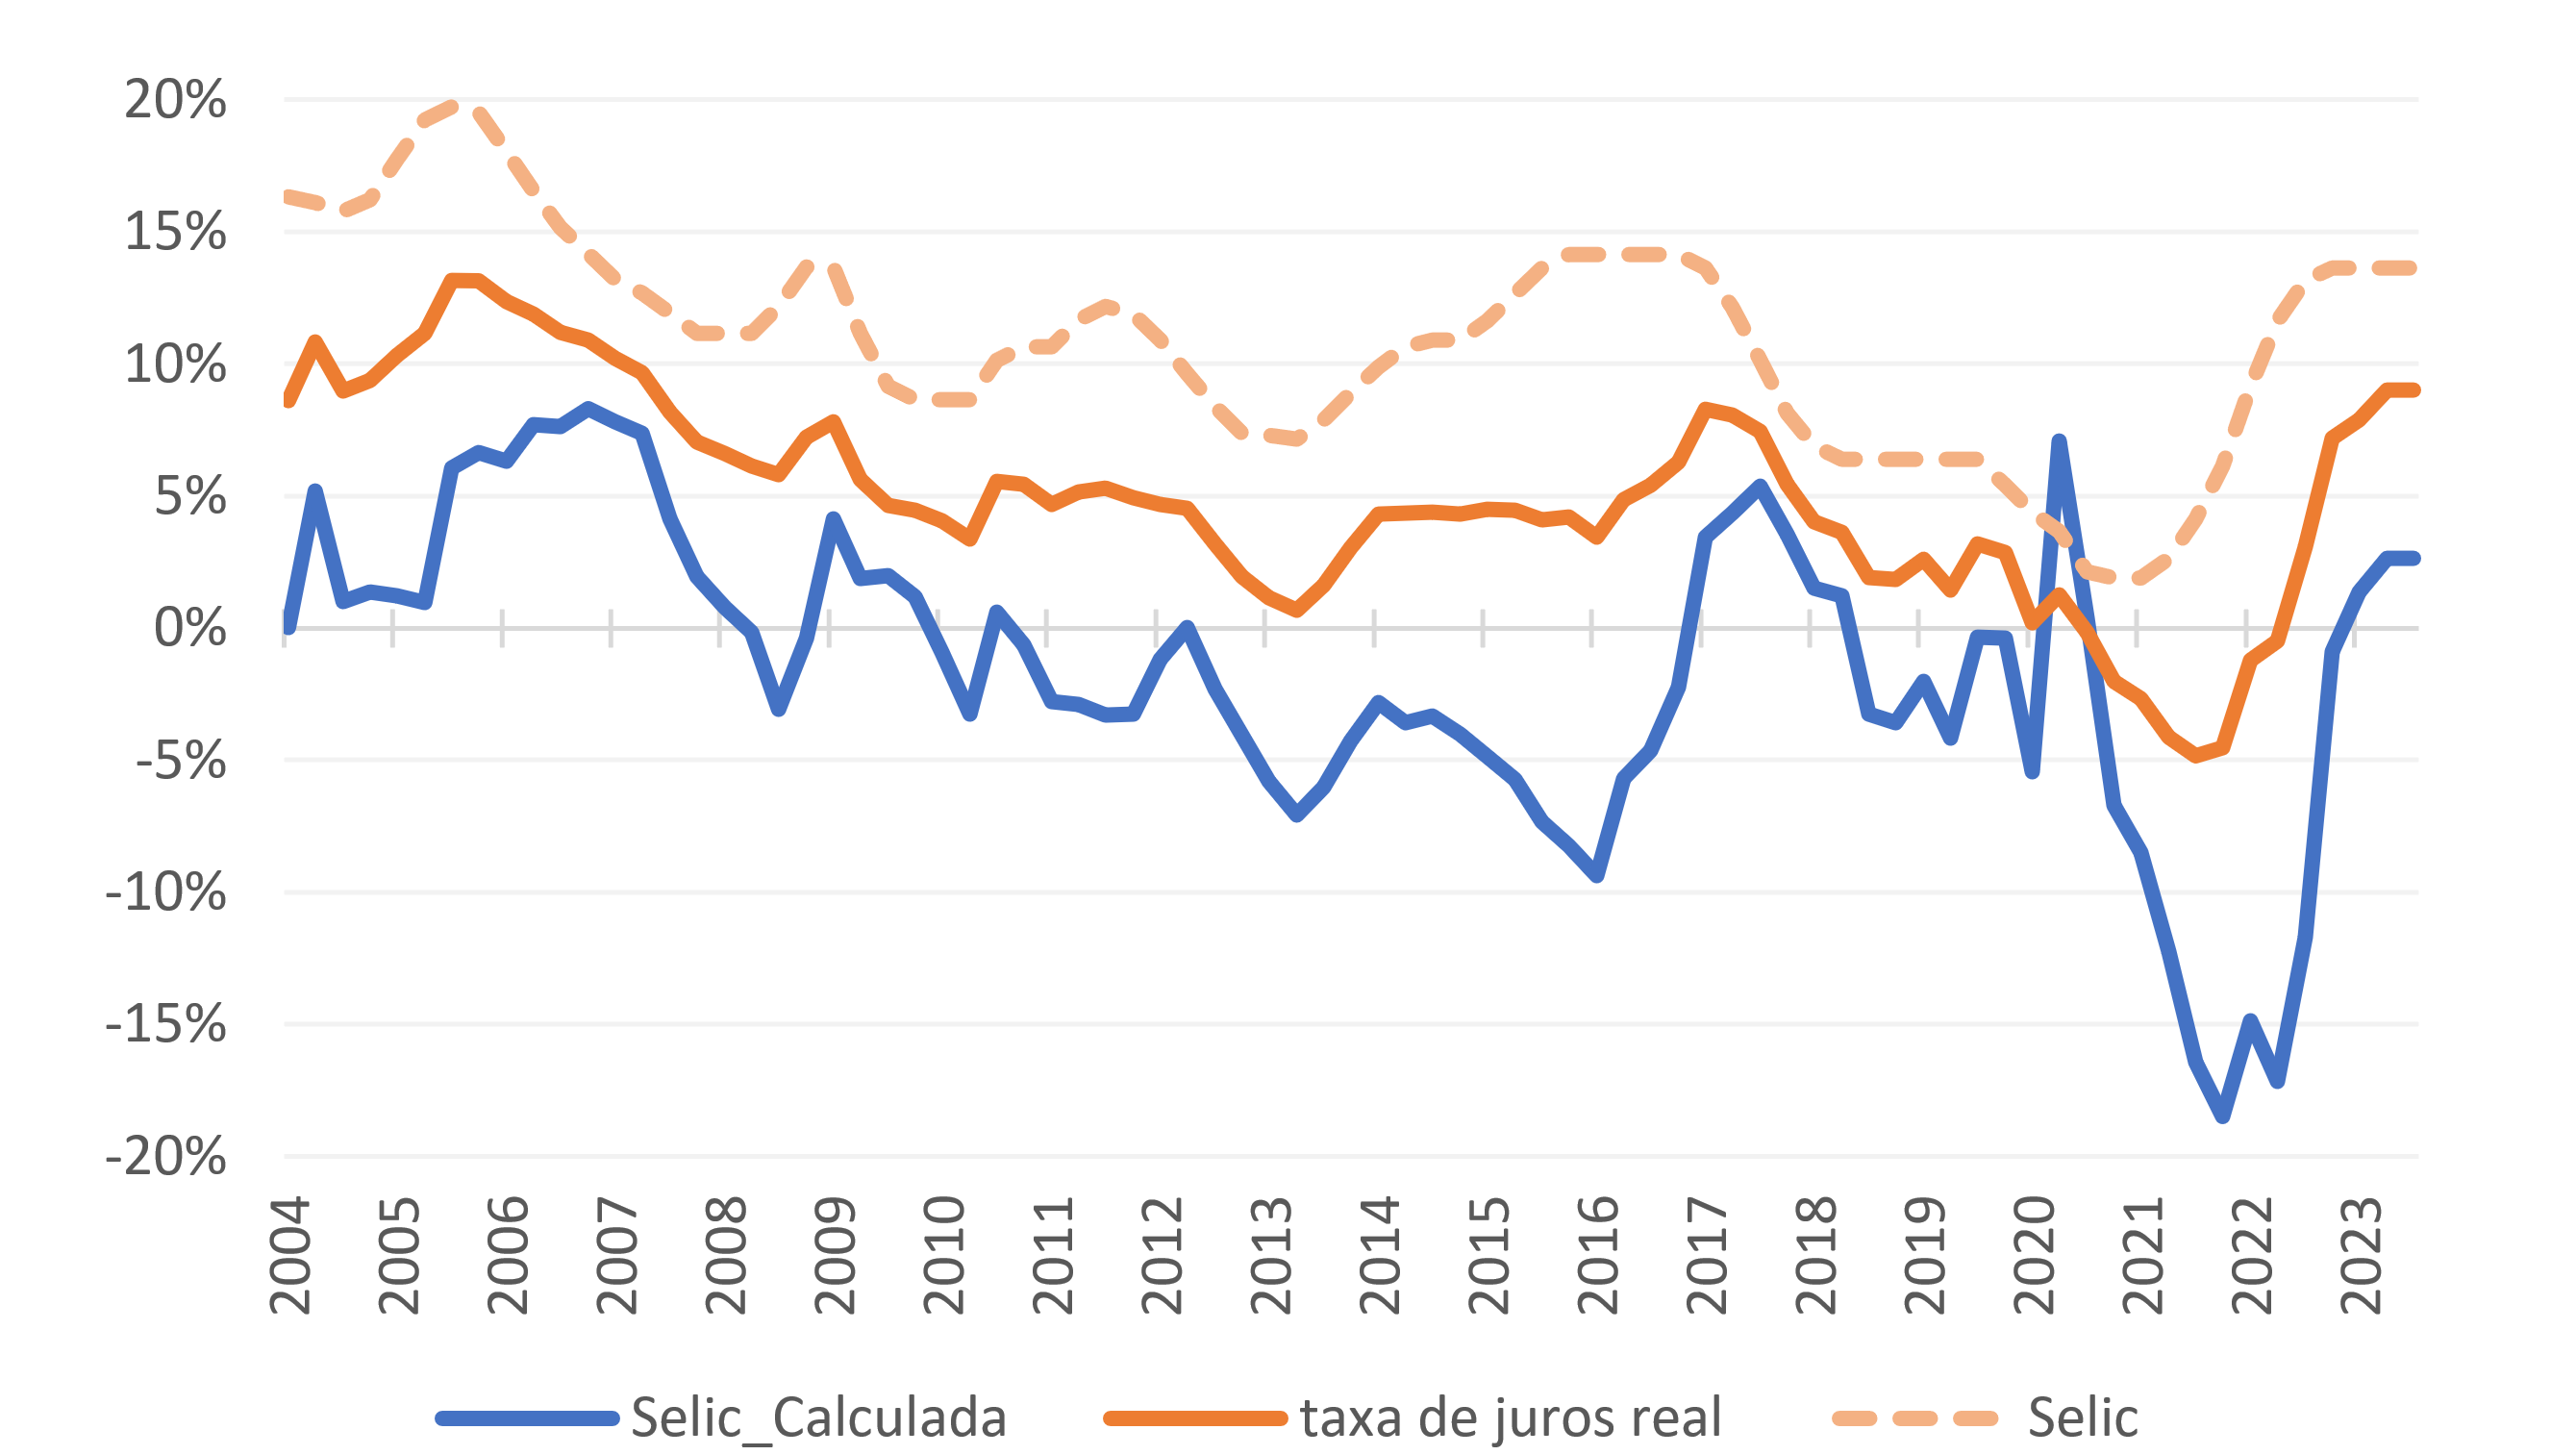
\includegraphics[width = .9\linewidth]{relatorios/macro/imagens/grafico4}
\end{figure}

\begin{figure}
    \centering
    \caption{Taxas de juros estado-unidenses}
    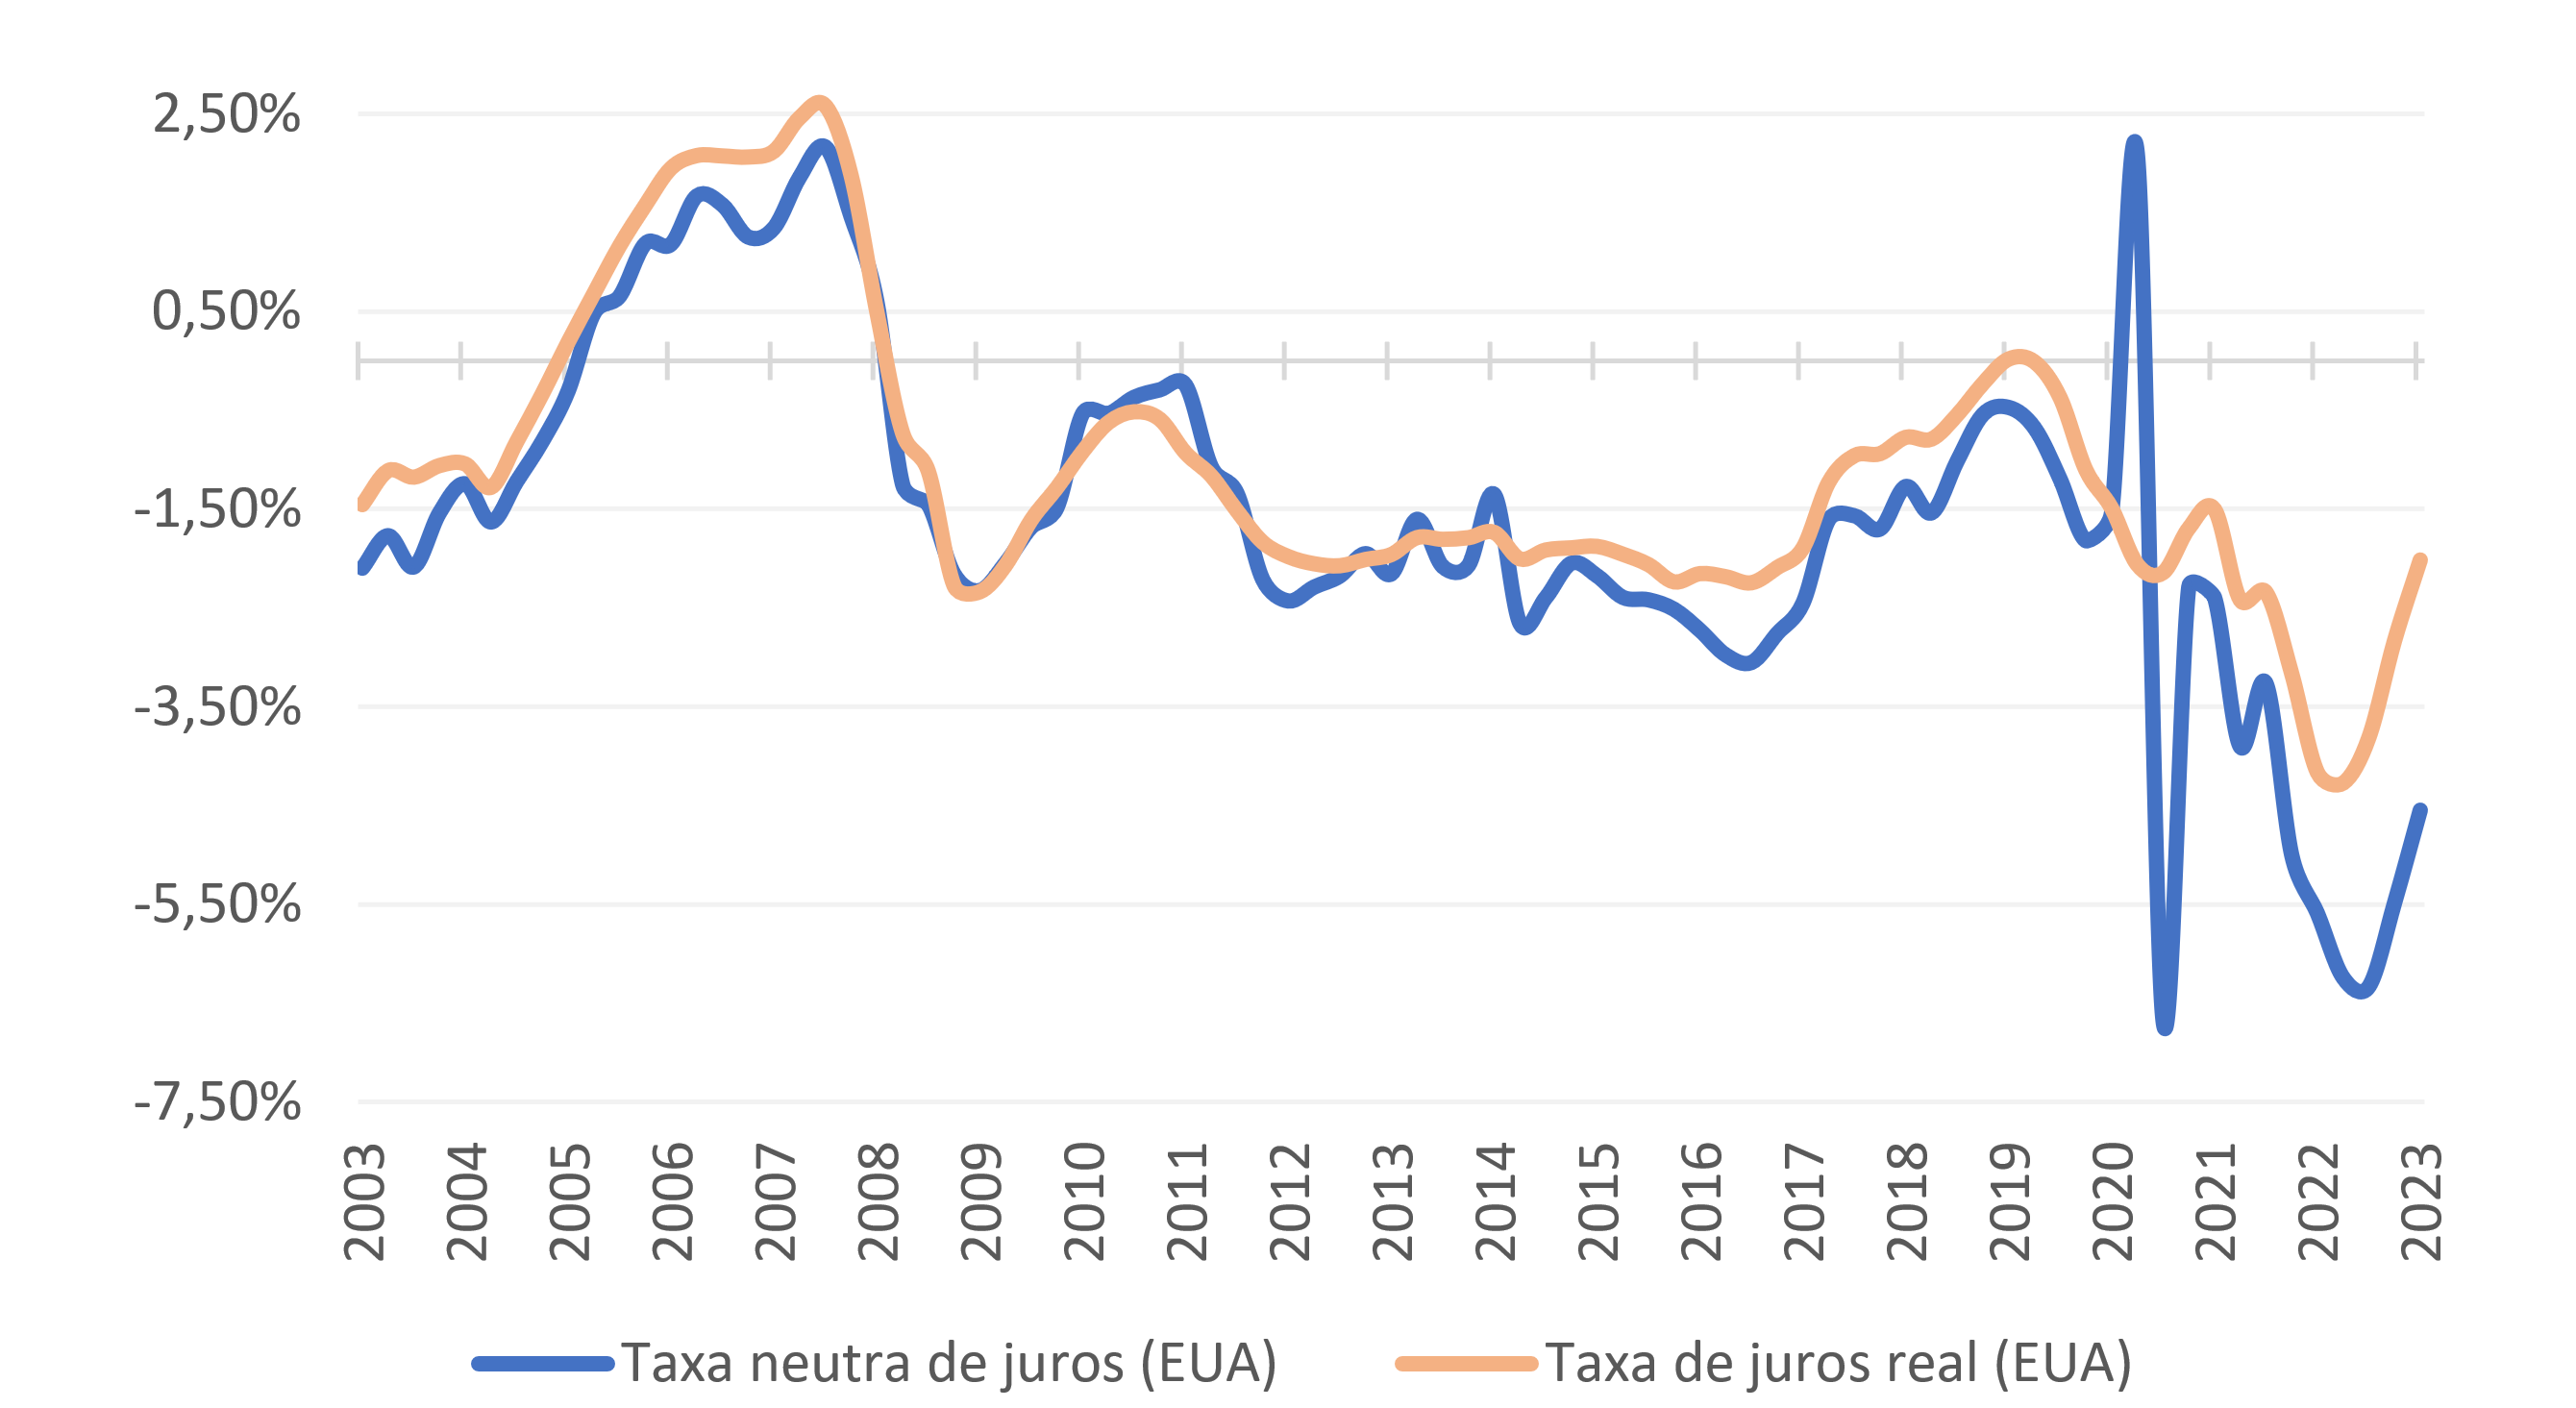
\includegraphics[width = .9\linewidth]{relatorios/macro/imagens/grafico5}
\end{figure}

Tem-se como resultado uma clara disparidade entre a dist\^{a}ncia da taxa de juros neutra com as taxas de juros reais respectivas dos pa\'{i}ses. \'{E} importante destacar que, nos EUA, por se tratar de um pa\'{i}s com uma economia desenvolvida e consequentemente mais est\'{a}vel, estes abordam o determinado Zero Lower Bound, um m\'{e}todo de determina\c{c}\~{a}o da taxa de juros efetiva o qual consiste em manter suas taxas nominais acima de zero, uma vez que em muitos per\'{i}odos de baix\'{i}ssima infla\c{c}\~{a}o, c\'{a}lculos para a taxa de juros ideal indiquem que uma adequada seria abaixo de zero, por\'{e}m a Zero Lower Bound, tamb\'{e}m abordada por diversos pa\'{i}ses europeus, impede que as taxas fiquem negativas, pois tal contradiz os princ\'{i}pios econ\^{o}micos da taxa de juros. Com isso, para melhor observa\c{c}\~{a}o dos dados, n\~{a}o foi inclu\'{i}do no gr\'{a}fico a taxa de juros nominal dos EUA, uma vez que esta se distanciaria da taxa neutra por imposi\c{c}\~{o}es de valores alterados externamente. 

 Tendo em vista os resultados observados nos gr\'{a}ficos 4 e 5, e sabendo que \'{e} a partir da diferen\c{c}a entre a taxa de juros real e a taxa real neutra de juros que conseguimos avaliar a qu\~{a}o apertada (ou relaxada) est\'{a} a pol\'{i}tica monet\'{a}ria, entendemos que o Brasil possui a tend\^{e}ncia de ter sua pol\'{i}tica muito mais apertada do que os Estados Unidos, ou seja, o Banco Central do Brasil imp\~{o}es pol\'{i}ticas para restringir a quantidade de moeda em circula\c{c}\~{a}o muito mais do que qualquer outro pa\'{i}s. 

 Para identificarmos as raz\~{o}es das pol\'{i}ticas monet\'{a}rias brasileiras se diferenciarem das do restante do globo, seria necess\'{a}rio entender quais os fatores ex\'{o}genos que influenciam a necessidade de impor uma taxa de juros t\~{a}o elevada para que uma pol\'{i}tica contracionista entre efetivamente em vigor na sociedade brasileira. As hip\'{o}teses mais frequentes seriam a confiabilidade no banco central, a quantidade e divulga\c{c}\~{a}o de intrigas pol\'{i}ticas e a influ\^{e}ncia de vari\'{a}veis externas ao pa\'{i}s, tendo em vista o grupo de controle, podemos considerar que uma das disparidades da sociedade americana da brasileira seria o apoio ou confian\c{c}a por parte da popula\c{c}\~{a}o nas autoridades p\'{u}blicas, o que pode afetar as decis\~{o}es financeiras dos indiv\'{i}duos impactando a economia como um todo. 

 Em contrapartida, analisando as oscila\c{c}\~{o}es presentes na taxa de juros neutra ao longo dos anos, sabemos que esta possui uma tend\^{e}ncia favor\'{a}vel \`{a} queda quando se trata de um per\'{i}odo com maior grau de compromisso com metas fiscais, aprova\c{c}\~{a}o de reformas estruturais, publica\c{c}\~{a}o de mat\'{e}rias relacionadas \`{a} maior seguridade de trabalho, entre outros, como o per\'{i}odo de 2009 \`{a} 2016. J\'{a} as medidas que podem ser relacionadas ao movimento de aumento da taxa neutra s\~{a}o a eleva\c{c}\~{a}o da d\'{i}vida p\'{u}blica e o fator ex\'{o}geno do mercado internacional que sensibiliza o modelo nacional no mesmo sentido, como ao longo de 2016 e 2017.  

\section*{Limita\c{c}\~{o}es }

 No trabalho descrito realizado pelo grupo, reconhece-se que o m\'{e}todo de determina\c{c}\~{a}o da taxa neutra de juros pode estar equivocado no sentido que, dado por se tratar de uma vari\'{a}vel utilizada de diferentes formas pelas economias ao redor do globo, \'{e} ineficiente determinar uma f\'{o}rmula capaz de sumarizar todos os fatores influentes para essas economias, como a natureza discricion\'{a}ria dos \textit{policy makers}, a fim de encontrar uma taxa neutra compar\'{a}vel entre todos. Por\'{e}m, m\'{e}todos aproximados que generalizam esses fatores como a Regra de Taylor, ainda podem ser aceitos dados que o objeto deste trabalho \'{e} uma compara\c{c}\~{a}o simples das varia\c{c}\~{o}es hist\'{o}ricas de duas taxas. 

 Visto isso, \'{e} importante destacar tamb\'{e}m as vari\'{a}veis ex\'{o}genas que foram desconsideradas na estipula\c{c}\~{a}o da f\'{o}rmula, como a confiabilidade no BC, j\'{a} que se trata de uma vari\'{a}vel qualitativa sendo impratic\'{a}vel sua introdu\c{c}\~{a}o em uma f\'{o}rmula. S\~{a}o estas e outras limita\c{c}\~{o}es que podem ser reconhecidas no modelo descrito no presente trabalho j\'{a} que se trata de dois pa\'{i}ses com sociedades diferentes com fatores psicol\'{o}gicos e ambientais distintos, por\'{e}m elas n\~{a}o s\~{a}o vistas como impeditivas para a an\'{a}lise apresentada. 

 \printbibliography[keyword = macro]
